\documentclass{tufte-handout}
\usepackage{pgfplots}
\usepackage[dvipsnames]{xcolor}
\usepackage{ulem}
\usepackage{subcaption}
\usepackage{amssymb, amsmath, pgfplots, tabularx, siunitx}
\usepackage{algorithm}
\usepackage{algorithmic}
\usepackage{makecell}
\usepackage{amsfonts}
\usepackage{thmtools}
\usepackage{enumitem}
\usepackage{adjustbox}
\usepackage{listings}
\usepackage{booktabs}
\pgfplotsset{compat = newest}

\usepackage{tikz}
\usetikzlibrary{shadings}
\usetikzlibrary{calc,arrows.meta}
\usetikzlibrary{shapes.misc}
\usetikzlibrary{shapes.geometric}
\usetikzlibrary{matrix}
\usetikzlibrary{positioning}
\usetikzlibrary{decorations.pathmorphing}
\usepackage[most]{tcolorbox}
\usepgfplotslibrary{colormaps,patchplots}

% Cores preservadas
\definecolor{wp-bg}{HTML}{FDF6EF}
\definecolor{wp-text}{HTML}{2D1B0E}
\definecolor{wp-primary}{HTML}{C24A3A}
\definecolor{wp-accent}{HTML}{D4952E}
\definecolor{wp-light}{HTML}{F0DECA}
\definecolor{wp-muted}{HTML}{C4A88A}
\definecolor{wp-dark}{HTML}{1A0F07}
\definecolor{wp-code}{HTML}{FDF2E4}

\pagecolor{wp-bg}
\color{wp-text}

\hypersetup{colorlinks=true,linkcolor=wp-primary,urlcolor=wp-accent}

\let\subsubsection\subsection

% Theorem environments
\declaretheorem[style=plain, name=Definition, numberwithin=section]{defn}
\declaretheorem[style=plain, name=Theorem, numberwithin=section]{thm}
\declaretheorem[style=plain, name=Lemma, numberwithin=section]{lem}
\declaretheorem[style=remark, name=Example, numberwithin=section]{exmp}
\declaretheorem[style=remark, name=Remark, numberwithin=section]{remark}

% Configuração do listings
\lstdefinestyle{pythonstyle}{
    language=Python,
    backgroundcolor=\color{wp-code},
    basicstyle=\ttfamily\small\color{wp-text},
    keywordstyle=\color{wp-primary}\bfseries,
    stringstyle=\color{wp-accent},
    commentstyle=\color{wp-muted}\itshape,
    numbers=left,
    numberstyle=\tiny\color{wp-muted},
    numbersep=8pt,
    breaklines=true,
    frame=single,
    rulecolor=\color{wp-muted!50},
    framerule=0.5pt,
    xleftmargin=15pt,
    showstringspaces=false
}
\lstset{style=pythonstyle}

\title{Machine Learning Notes \\ Chapter 2: Differentiable Programming and Optimization}
\author{Vitor N. Cabral de Oliveira\\ \href{mailto:vnco@cin.ufpe.br}{vnco@cin.ufpe.br}}
\date{\today}

\begin{document}
\maketitle
\begin{abstract}
    In Chapter 1, we established the forward pass—the mechanism by which a neural network transforms inputs into predictions. However, the network was static, relying on random initialization. In this chapter, we unlock the engine of learning. We explore how neural networks evaluate the impact of every parameter on the final error using differentiable programming (Autograd) and how they navigate the complex landscape of the loss function using optimization algorithms. We will build a miniature automatic differentiation engine from scratch to demystify the \texttt{.backward()} call found in modern frameworks.
\end{abstract}

\newpage
\hypersetup{linkcolor=wp-text}
\tableofcontents
\hypersetup{linkcolor=wp-primary}
\newpage

\section{Part I: The Engine (Differentiable Programming)}

To teach our model to learn, we must answer a fundamental question: \textit{If I change this specific weight by a tiny amount, how much will the total error change?} The mathematical tool to answer this is the derivative. However, neural networks have millions of parameters nested in complex compositions. Calculating these derivatives manually is infeasible. This is where Automatic Differentiation (Autodiff) comes in.

\subsection{The Calculus of Compositions: The Chain Rule}

The foundation of autodiff is the chain rule from calculus. If a scalar variable $L$ depends on $y$, and $y$ depends on $x$, the rate of change of $L$ with respect to $x$ is the product of the local rates of change:
\[
\frac{\partial L}{\partial x} = \frac{\partial L}{\partial y} \frac{\partial y}{\partial x}
\]
A neural network is simply a massive composition of functions: $L = f_n(f_{n-1}(\dots f_1(\mathbf{x})\dots))$. The chain rule allows us to decompose the gradient of the loss with respect to the inputs into a product of local gradients calculated at each layer.

\subsubsection{The Multivariable Chain Rule (The Sum Rule)}

In deep learning, a parameter often influences the loss through \textit{multiple paths} in the network. Suppose $L$ depends on $y_1$ and $y_2$, and both $y_1$ and $y_2$ depend on $x$. The total derivative of $L$ with respect to $x$ is the sum of the derivatives along each path:
\[
\frac{\partial L}{\partial x} = \frac{\partial L}{\partial y_1} \frac{\partial y_1}{\partial x} + \frac{\partial L}{\partial y_2} \frac{\partial y_2}{\partial x}
\]
This "sum rule" is critical. It means that during backpropagation, if a node receives gradients from multiple downstream paths, those gradients must be \textbf{accumulated} (summed) to find the true gradient.

\begin{exmp}[A Variable That Appears Twice]
Consider the expression $L = x^2 + x$ and suppose $x = 3$. Here $x$ reaches the loss through two paths: the branch $y_1 = x^2$ and the branch $y_2 = x$. The local derivatives are
\[
\frac{\partial y_1}{\partial x} = 2x = 6, \qquad \frac{\partial y_2}{\partial x} = 1.
\]
Since $L = y_1 + y_2$, both branches connect directly to the root with $\frac{\partial L}{\partial y_1} = \frac{\partial L}{\partial y_2} = 1$. The chain rule says we must \emph{add} the contributions of every path:
\[
\frac{\partial L}{\partial x} = \frac{\partial L}{\partial y_1}\frac{\partial y_1}{\partial x} + \frac{\partial L}{\partial y_2}\frac{\partial y_2}{\partial x} = 1 \cdot 6 + 1 \cdot 1 = 7.
\]
We can verify analytically: $\frac{d}{dx}(x^2 + x) = 2x + 1 = 7$ at $x = 3$. Had we kept only one path, we would have obtained $6$ or $1$---both wrong. This is precisely why the \texttt{Valor} engine accumulates with \texttt{+=}: a parameter that is reused by many paths must receive the gradient from every one of them.
\end{exmp}

\subsection{Computational Graphs}

To automate the application of the chain rule, we represent the mathematical expressions as a \textbf{Computational Graph}—a Directed Acyclic Graph (DAG) where nodes are operations (or variables), and edges represent the flow of data.

\begin{marginfigure}[-6.0cm]
\centering
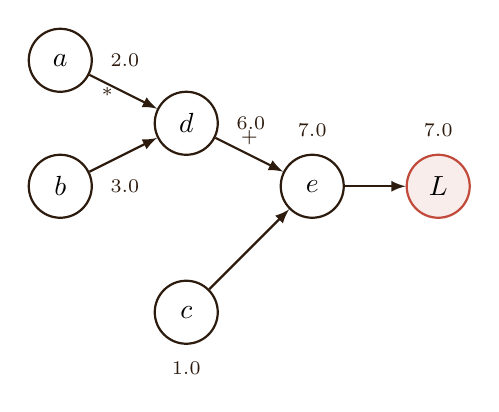
\begin{tikzpicture}[scale=0.8, >=latex, node distance=1.5cm]
    % Inputs
    \node[circle, draw=wp-text, thick, minimum size=0.8cm] (a) at (0,2) {$a$};
    \node[circle, draw=wp-text, thick, minimum size=0.8cm] (b) at (0,0) {$b$};
    \node[circle, draw=wp-text, thick, minimum size=0.8cm] (c) at (2,-2) {$c$};
    
    % Ops
    \node[circle, draw=wp-text, thick, minimum size=0.8cm] (d) at (2,1) {$d$};
    \node[circle, draw=wp-text, thick, minimum size=0.8cm] (e) at (4,0) {$e$};
    
    % Root
    \node[circle, draw=wp-primary, thick, fill=wp-primary!10, minimum size=0.8cm] (L) at (6,0) {$L$};
    
    % Edges
    \draw[->, wp-text, thick] (a) -- (d) node[midway, left, font=\scriptsize] {$*$};
    \draw[->, wp-text, thick] (b) -- (d);
    \draw[->, wp-text, thick] (d) -- (e) node[midway, above, font=\scriptsize] {$+$};
    \draw[->, wp-text, thick] (c) -- (e);
    \draw[->, wp-text, thick] (e) -- (L);
    
    % Values
    \node[wp-text, font=\scriptsize, right=0.1cm of a] {$2.0$};
    \node[wp-text, font=\scriptsize, right=0.1cm of b] {$3.0$};
    \node[wp-text, font=\scriptsize, below=0.1cm of c] {$1.0$};
    \node[wp-text, font=\scriptsize, right=0.1cm of d] {$6.0$};
    \node[wp-text, font=\scriptsize, above=0.1cm of e] {$7.0$};
    \node[wp-text, font=\scriptsize, above=0.1cm of L] {$7.0$};
\end{tikzpicture}
\caption{A computational graph for $L = (a \times b) + c$. Data flows forward (left to right). Gradients flow backward.}
\label{fig:comp_graph}
\end{marginfigure}

Consider the expression $L = (a \times b) + c$. In a graph, inputs ($a, b, c$) are leaves, $d = a \times b$ is an intermediate node, $e = d + c$ is another, and $L = e$ is the root. The \textit{forward pass} evaluates the graph from leaves to root, storing intermediate results.

\subsection{Backpropagation is Reverse-Mode Autodiff}

\textbf{Backpropagation} is simply the application of the chain rule to this graph in reverse—from the root (Loss) back to the leaves (Weights). We traverse the graph in \textbf{topological order}, ensuring that when we compute the gradient for a node, we have already accumulated all gradients from its children.

Let's trace it manually for Figure~\ref{fig:comp_graph}:
\begin{enumerate}[leftmargin=*, itemsep=2pt]
    \item \textbf{At the root:} $\frac{\partial L}{\partial L} = 1.0$. We seed the graph with a gradient of $1.0$.
    \item \textbf{At node $e$:} Since $L = e$, locally $\frac{\partial L}{\partial e} = 1.0$. We pass this gradient backward.
    \item \textbf{At node $d$ and $c$ (from $e$):} The operation is $e = d + c$. The local derivatives are $\frac{\partial e}{\partial d} = 1$ and $\frac{\partial e}{\partial c} = 1$. By the chain rule, $\frac{\partial L}{\partial d} = \frac{\partial L}{\partial e} \times 1 = 1.0$, and $\frac{\partial L}{\partial c} = \frac{\partial L}{\partial e} \times 1 = 1.0$.
    \item \textbf{At node $a$ and $b$ (from $d$):} The operation is $d = a \times b$. The local derivatives are $\frac{\partial d}{\partial a} = b$ and $\frac{\partial d}{\partial b} = a$. Applying the chain rule: $\frac{\partial L}{\partial a} = \frac{\partial L}{\partial d} \times b = 1.0 \times 3.0 = 3.0$, and $\frac{\partial L}{\partial b} = \frac{\partial L}{\partial d} \times a = 1.0 \times 2.0 = 2.0$.
\end{enumerate}

\subsection{A Complete Numeric Walkthrough}

To make the mechanism concrete, let us execute the entire forward and backward pass for the graph in Figure~\ref{fig:comp_graph}, step by step, tracking the values as a computer would.

\textbf{Forward pass} (evaluate leaves $\rightarrow$ root, caching each intermediate value):

\begin{table}[htbp]
\centering
\small
\begin{tabular}{@{}clcl@{}}
\toprule
\textbf{Step} & \textbf{Operation} & \textbf{Value} & \textbf{Stored in} \\
\midrule
1 & $a = 2.0$ & $2.0$ & node $a$ \\
2 & $b = 3.0$ & $3.0$ & node $b$ \\
3 & $c = 1.0$ & $1.0$ & node $c$ \\
4 & $d = a \times b$ & $2.0 \times 3.0 = 6.0$ & node $d$ \\
5 & $e = d + c$ & $6.0 + 1.0 = 7.0$ & node $e$ \\
6 & $L = e$ & $7.0$ & node $L$ \\
\bottomrule
\end{tabular}
\caption{Forward pass for $L = (a \times b) + c$ with $a=2.0$, $b=3.0$, $c=1.0$.}
\label{tab:forward_walk}
\end{table}

\textbf{Backward pass} (reverse order, accumulating $\frac{\partial L}{\partial \cdot}$ at each node):

\begin{table}[htbp]
\centering
\small
\begin{tabular}{@{}clcl@{}}
\toprule
\textbf{Node} & \textbf{Local derivative} & \textbf{Incoming} $\frac{\partial L}{\partial \cdot}$ & \textbf{Gradient} \\
\midrule
$L$ & seed: $\frac{\partial L}{\partial L} = 1.0$ & --- & $1.0$ \\
$e$ & $\frac{\partial e}{\partial e} = 1.0$ & $\frac{\partial L}{\partial e} = 1.0$ & $1.0$ \\
$c$ & $\frac{\partial e}{\partial c} = 1.0$ & $\frac{\partial L}{\partial e} = 1.0$ & $1.0 \times 1.0 = 1.0$ \\
$d$ & $\frac{\partial e}{\partial d} = 1.0$ & $\frac{\partial L}{\partial e} = 1.0$ & $1.0 \times 1.0 = 1.0$ \\
$b$ & $\frac{\partial d}{\partial b} = a = 2.0$ & $\frac{\partial L}{\partial d} = 1.0$ & $1.0 \times 2.0 = 2.0$ \\
$a$ & $\frac{\partial d}{\partial a} = b = 3.0$ & $\frac{\partial L}{\partial d} = 1.0$ & $1.0 \times 3.0 = 3.0$ \\
\bottomrule
\end{tabular}
\caption{Backward pass: each node multiplies its local derivative by the incoming gradient.}
\label{tab:backward_walk}
\end{table}

The final gradients are exactly what we derived by hand. The gradient $\left(\frac{\partial L}{\partial a}, \frac{\partial L}{\partial b}, \frac{\partial L}{\partial c}\right) = (3.0, 2.0, 1.0)$ tells us the sensitivity of the loss to each input: perturbing $a$ by a tiny amount $\epsilon$ changes $L$ by about $3\epsilon$, perturbing $b$ by $2\epsilon$, and perturbing $c$ by only $\epsilon$. In training, this is precisely the information used to decide how much each parameter should move.

The magic of Autodiff is that we don't write these equations manually. The framework builds the graph dynamically during the forward pass and traverses it in reverse to multiply and accumulate the local gradients automatically.

\subsection{Forward-Mode vs. Reverse-Mode Autodiff}

Backpropagation is one of two classical strategies for automatic differentiation. Understanding the alternative clarifies why neural networks use reverse mode.

\subsubsection{Forward-Mode Autodiff (Dual Numbers)}

Instead of storing a single number $x$, forward mode attaches to it a \textbf{dual number} $x + \dot{x}\,\varepsilon$, where $\varepsilon$ is a formal symbol with $\varepsilon^2 = 0$. The component $\dot{x}$ tracks the derivative of $x$ along a chosen direction. Arithmetic on dual numbers propagates derivatives for free:
\[
(x + \dot{x}\varepsilon) + (y + \dot{y}\varepsilon) = (x+y) + (\dot{x}+\dot{y})\varepsilon,
\]
\[
(x + \dot{x}\varepsilon) \cdot (y + \dot{y}\varepsilon) = (xy) + (\dot{x}y + x\dot{y})\varepsilon.
\]
Notice the $\varepsilon$-component of a product is exactly the product rule. If we seed $\dot{x} = 1$ for one input and $\dot{x} = 0$ for the others, a single forward pass computes $\frac{\partial L}{\partial x}$ for that one input. Computing the full gradient $\nabla_\theta \mathcal{L}$ over $n$ parameters therefore requires $n$ forward passes.

\subsubsection{Reverse-Mode Autodiff (Backpropagation)}

Backpropagation is the mirror image: it propagates derivatives from the output backward to the inputs. One forward pass evaluates all values; one backward pass computes the derivative with respect to \emph{every} input simultaneously. Crucially, the cost of the backward pass is proportional to the number of edges in the graph---roughly the same as the forward pass---regardless of how many inputs there are.

\begin{remark}[Why Reverse Mode Wins]
A neural network has millions of parameters $\theta$ (inputs to the derivative) but only \emph{one} scalar loss $\mathcal{L}$ (the output). Forward mode would need $n$ passes for $n$ parameters; reverse mode needs exactly two. This single fact is why every deep learning framework computes gradients by backpropagation.
\end{remark}

\begin{table}[htbp]
\centering
\small
\begin{tabularx}{\textwidth}{@{}>{\raggedright\arraybackslash}p{3.0cm}X X@{}}
\toprule
 & \textbf{Forward Mode} & \textbf{Reverse Mode} \\
\midrule
What it computes & Derivative along one input direction & Derivative w.r.t.\ all inputs \\
Passes for $n$ inputs & $n$ forward passes & 1 forward + 1 backward \\
Cost & $O(n \times \text{graph size})$ & $O(\text{graph size})$ \\
Best when & Few inputs, many outputs & Few outputs, many inputs \\
Deep learning & $n$ = millions $\Rightarrow$ hopeless & Exactly the training scenario \\
\bottomrule
\end{tabularx}
\caption{Comparing forward-mode and reverse-mode automatic differentiation. Reverse mode is what PyTorch implements in \texttt{backward()}.}
\label{tab:fwd_vs_rev}
\end{table}

\subsection{Implementing the "Micrograd"}

To truly demystify PyTorch's \texttt{.backward()}, we will build a minimal autograd engine. We create a \texttt{Valor} class that stores both the data and its gradient. When we perform operations on \texttt{Valor} objects, we dynamically build the computational graph.

\begin{lstlisting}[caption={The \texttt{Valor} class in \texttt{mini\_nn/autograd.py}.}]
import numpy as np

class Valor:
    def __init__(self, data, _children=(), _op=''):
        self.data = data
        self.grad = 0
        # Internal variables for autograd graph
        self._prev = set(_children)
        self._op = _op
        self._backward = lambda: None # Local gradient function

    def __repr__(self):
        return f"Valor(data={self.data:.4f}, grad={self.grad:.4f})"

    def __add__(self, other):
        # Ensure other is a Valor object
        other = other if isinstance(other, Valor) else Valor(other)
        out = Valor(self.data + other.data, (self, other), '+')

        def _backward():
            # d(out)/d(self) = 1, d(out)/d(other) = 1
            # We use += to accumulate gradients from multiple paths
            self.grad += 1.0 * out.grad
            other.grad += 1.0 * out.grad
        out._backward = _backward
        return out

def __mul__(self, other):
        other = other if isinstance(other, Valor) else Valor(other)
        out = Valor(self.data * other.data, (self, other), '*')

        def _backward():
            # d(out)/d(self) = other, d(out)/d(other) = self
            self.grad += other.data * out.grad
            other.grad += self.data * out.grad
        out._backward = _backward
        return out

    def __neg__(self):
        # Negation is just multiplication by -1
        return self * -1

    def __sub__(self, other):
        # Subtraction is addition of a negated term
        return self + (-other)

    def __rsub__(self, other):
        # Handles expressions like 5 - x
        return other + (-self)

    def __truediv__(self, other):
        # Division is multiplication by the inverse power
        return self * other ** -1

    def __pow__(self, other):
        # only supports integer/float exponents
        assert isinstance(other, (int, float)), "only constant powers"
        out = Valor(self.data ** other, (self,), f'**{other}')

        def _backward():
            # d(x^n)/dx = n * x^(n-1)
            self.grad += (other * self.data ** (other - 1)) * out.grad
        out._backward = _backward
        return out

    def exp(self):
        x = self.data
        out = Valor(np.exp(x), (self,), 'exp')

        def _backward():
            # d(exp(x))/dx = exp(x)
            self.grad += out.data * out.grad
        out._backward = _backward
        return out

    def relu(self):
        x = self.data
        out = Valor(x if x > 0 else 0, (self,), 'relu')

        def _backward():
            # d(relu(x))/dx = 1 if x > 0 else 0
            self.grad += (out.data > 0) * out.grad
        out._backward = _backward
        return out

    def sigmoid(self):
        x = self.data
        s = 1 / (1 + np.exp(-x))
        out = Valor(s, (self,), 'sigmoid')

        def _backward():
            # d(sigmoid(x))/dx = sigmoid(x) * (1 - sigmoid(x))
            self.grad += s * (1 - s) * out.grad
        out._backward = _backward
        return out

    def tanh(self):
        x = self.data
        t = (np.exp(2*x) - 1) / (np.exp(2*x) + 1)
        out = Valor(t, (self,), 'tanh')

        def _backward():
            # d(tanh)/dx = 1 - tanh(x)^2
            self.grad += (1 - t**2) * out.grad
        out._backward = _backward
        return out
\end{lstlisting}

Every operation follows the same pattern: (1) build the output node from the inputs, (2) register the inputs as children, (3) define a \texttt{\_backward} closure that implements the \emph{local} derivative, and (4) attach it. Once an operation is defined, all the others compose through it---for example, subtraction is ``add a negation'' and division is ``multiply by the inverse.'' This composability is the whole trick: \emph{any} differentiable function can be built from a small set of primitive operations.

\begin{remark}[The \texttt{+=} Accumulation]
Notice the use of \texttt{+=} in the \texttt{\_backward} functions. If a node is used multiple times in a graph (e.g., $y = x \times x$), the gradients from all paths must be summed. This is a direct application of the multivariable chain rule (the sum rule). Without \texttt{+=}, gradients would be overwritten instead of accumulated, leading to incorrect optimization.
\end{remark}

\subsection{Topological Sort and the Backward Pass}

To execute the backward pass, we must traverse the graph such that a node is processed only after all of its children have been processed. This ordering is called a \textbf{Topological Sort}. 

\begin{lstlisting}[caption={The \texttt{backward} method using topological sort.}]
    def backward(self):
        # Build topological order (root must be last)
        topo = []
        visited = set()
        
        def build_topo(v):
            if v not in visited:
                visited.add(v)
                for child in v._prev:
                    build_topo(child)
                topo.append(v)
                
        build_topo(self)

        # Seed the root gradient to 1.0
        self.grad = 1.0
        
        # Call backward() in reverse topological order
        for v in reversed(topo):
            v._backward()
\end{lstlisting}

This algorithm recursively visits children before parents, appending them to a list. By iterating over this list in reverse, we guarantee that when we calculate the local gradients of a node, the gradient flowing into it (\texttt{out.grad}) has already been fully accumulated.

\subsection{Building a Network with Valor}

We now have an engine that can differentiate any scalar expression. To build a neural network, we assemble \texttt{Valor} nodes into neurons and layers. Each neuron holds a vector of weights and a bias---all \texttt{Valor} objects---and computes the usual affine transformation followed by an activation:

\begin{lstlisting}[caption={A neuron, layer, and MLP built from \texttt{Valor} in \texttt{mini\_nn/network.py}.}]
class Neuron:
    def __init__(self, nin):
        # nin = number of inputs; weights and bias are trainable Valor nodes
        self.w = [Valor(np.random.uniform(-1, 1)) for _ in range(nin)]
        self.b = Valor(0.0)

    def __call__(self, x):
        # z = sum(w_i * x_i) + b, then apply tanh
        z = sum((wi * xi for wi, xi in zip(self.w, x)), self.b)
        return z.tanh()

    def parameters(self):
        return self.w + [self.b]

class Layer:
    def __init__(self, nin, nout):
        self.neurons = [Neuron(nin) for _ in range(nout)]

    def __call__(self, x):
        return [n(x) for n in self.neurons]

    def parameters(self):
        return [p for neuron in self.neurons for p in neuron.parameters()]

class MLP:
    def __init__(self, sizes):
        # sizes = [2, 4, 1] means 2 inputs, 4 hidden neurons, 1 output
        self.layers = [Layer(sizes[i], sizes[i+1]) for i in range(len(sizes) - 1)]

    def __call__(self, x):
        for layer in self.layers:
            x = layer(x)          # outputs of one layer feed the next
        return x[0]               # scalar output (single output neuron)

    def parameters(self):
        return [p for layer in self.layers for p in layer.parameters()]
\end{lstlisting}

The beauty of this design is that the network is built \emph{the same way as any other expression}. Calling an MLP on an input $x$ performs the forward pass and silently constructs the computational graph. The \texttt{parameters()} method collects every \texttt{Valor} node that should be optimized---these are exactly the leaves whose gradients backpropagation will compute.

\subsection{A Complete Training Example}

Let us put everything together by training a small MLP to learn the \textbf{XOR} function, the classic example of a problem that a single perceptron cannot solve. The full training loop exercises every concept from Part I and Part II:

\begin{lstlisting}[caption={Training a 2-4-1 MLP on XOR. Each step is a mini-batch update via SGD.}]
# Dataset: XOR (2 inputs, 1 output)
xs = [[0,0], [0,1], [1,0], [1,1]]
ys = [0, 1, 1, 0]

# Build the model and collect all parameters
model = MLP([2, 4, 1])
params = model.parameters()

learning_rate = 1.0
for epoch in range(200):
    # ---- Forward pass ----
    preds = [model(x) for x in xs]

    # ---- Loss: mean squared error over the 4 examples ----
    loss = sum((y - pred) ** 2 for y, pred in zip(ys, preds)) / len(xs)

    # ---- Backward pass ----
    for p in params:
        p.grad = 0.0            # zero_grad: clear accumulated gradients
    loss.backward()

    # ---- Update: plain SGD ----
    for p in params:
        p.data -= learning_rate * p.grad

    if epoch % 40 == 0:
        print(f"epoch {epoch:3d} | loss {loss.data:.4f}")
\end{lstlisting}

\begin{remark}[Why \texttt{zero\_grad()}?]
Gradients \emph{accumulate} (the sum rule!). If we did not reset \texttt{p.grad} to zero before each \texttt{backward()}, the gradients from previous mini-batches would keep piling up, and every update would overshoot. In PyTorch this is exactly what \texttt{optimizer.zero\_grad()} does before \texttt{loss.backward()}.
\end{remark}

Over 200 epochs the loss decreases toward zero and the network learns the XOR mapping---even though the two inputs are not linearly separable. This tiny example contains the entire lifecycle of modern deep learning: forward pass, loss, backward pass, and a parameter update driven by the gradient.

\subsection{Transition to PyTorch}

Our \texttt{Valor} class is functionally identical to PyTorch's \texttt{torch.Tensor} in its autograd mechanics. When you call \texttt{loss.backward()} in PyTorch, it performs this exact reverse-mode autodiff on a highly optimized C++ graph. 

\subsubsection{From Scalars to Tensors: The Jacobian}

However, PyTorch operates on \textit{tensors} (multidimensional arrays) rather than scalars. The chain rule generalizes cleanly. If a function $\mathbf{f}: \mathbb{R}^n \to \mathbb{R}^m$ maps a vector input to a vector output, its derivative is no longer a single number but a matrix of all partial derivatives---the \textbf{Jacobian}:
\[
\mathbf{J}_{\mathbf{f}}(\mathbf{x}) = \begin{pmatrix}
\frac{\partial f_1}{\partial x_1} & \cdots & \frac{\partial f_1}{\partial x_n} \\
\vdots & \ddots & \vdots \\
\frac{\partial f_m}{\partial x_1} & \cdots & \frac{\partial f_m}{\partial x_n}
\end{pmatrix} \in \mathbb{R}^{m \times n}
\]
For a composition $\mathbf{h} = \mathbf{g} \circ \mathbf{f}$, the chain rule becomes a \emph{matrix product} of Jacobians:
\[
\mathbf{J}_{\mathbf{h}}(\mathbf{x}) = \mathbf{J}_{\mathbf{g}}(\mathbf{f}(\mathbf{x})) \cdot \mathbf{J}_{\mathbf{f}}(\mathbf{x})
\]
Exactly the same graph structure as before---each edge now carries a matrix instead of a scalar.

\subsubsection{Vector--Jacobian Products (VJPs)}

Naively, the backward pass would multiply full Jacobian matrices, which are enormous. Fortunately, we do not need the entire matrix. In reverse mode, the gradient flowing back is a vector $\mathbf{v}$, and what we need from each node is the \textbf{Vector--Jacobian Product}
\[
\mathbf{v}^{\mathsf{T}} \mathbf{J}_{\mathbf{f}}(\mathbf{x}).
\]
For any operation, autograd only needs to know how to multiply an incoming gradient vector by the operation's Jacobian---never to materialize the Jacobian itself. For elementwise operations (like $\tanh$ applied to every entry of a tensor), the Jacobian is diagonal and the VJP is just an elementwise product, which is why $\tanh$'s \texttt{\_backward} used $\mathbf{1}-\tanh^2$. This is the secret behind PyTorch's efficiency: \emph{scalar autodiff (our Valor) and tensor autodiff (PyTorch) are the same algorithm}, differing only in that the latter batches the arithmetic into matrices.

\begin{remark}[Gradients of Losses Are Always Vectors]
Because the loss $\mathcal{L}$ is a scalar, $\frac{\partial \mathcal{L}}{\partial \mathbf{x}}$ for any tensor $\mathbf{x}$ is a vector of the same shape as $\mathbf{x}$. This is why \texttt{param.grad} always ``looks like'' \texttt{param}. The scalar chain rule is simply applied entrywise through every tensor in the network.
\end{remark}

\section{Part II: The Steering Wheel (Optimization)}

Now that we possess the gradients—the vector pointing in the direction of steepest ascent of the loss—we must decide how to use this information to update the weights. This is the domain of optimization. If Autograd is the engine that calculates the slope, Optimization is the steering wheel that decides how fast and in what manner we descend the mountain.

\subsection{The Loss Landscape}

Imagine the loss function $\mathcal{L}(\theta)$ as a physical landscape in a space with millions of dimensions (one for each parameter in $\theta$). The goal of training is to find the coordinates $\theta^*$ that minimize this landscape (the lowest valley). The gradient $\nabla_\theta \mathcal{L}$ tells us the direction of the steepest uphill slope. Therefore, to descend, we step in the exact opposite direction: $-\nabla_\theta \mathcal{L}$.

\begin{marginfigure}[-2.0cm]
\centering
\begin{tcolorbox}[colback=wp-light, colframe=wp-accent, title=\textbf{Intuition: The Blind Hiker}]
Imagine a blindfolded hiker trying to reach the bottom of a valley. They feel the slope under their feet (the gradient) and take a step downhill (the update). The size of their step is the learning rate. If the step is too large, they might overshoot the valley and climb the opposite hill. If it's too small, they will never reach the bottom before winter.
\end{tcolorbox}
\end{marginfigure}

Unlike a smooth bowl, real loss landscapes contain rich structure that shapes how optimizers behave:

\begin{itemize}[leftmargin=*, itemsep=2pt]
    \item \textbf{Global/Local Minima:} The valleys we aim for. A \emph{local} minimum is the lowest point of its neighborhood but not necessarily of the whole landscape. Optimizers can get trapped in a local minimum and never find the global one.
    \item \textbf{Saddle Points:} Points where the slope is zero but which are neither a peak nor a valley---flat in one direction, sloping in another. Gradients vanish there, and plain SGD can stall for a long time.
    \item \textbf{Plateaus:} Large flat regions where gradients are near zero. Progress becomes extremely slow, which is why adaptive optimizers (which scale the step size) were invented.
    \item \textbf{Ravines:} Narrow, steep valleys where the surface curves sharply in one direction and gently in another. They cause plain SGD to oscillate violently across the walls.
\end{itemize}

\begin{figure}[htbp]
\centering
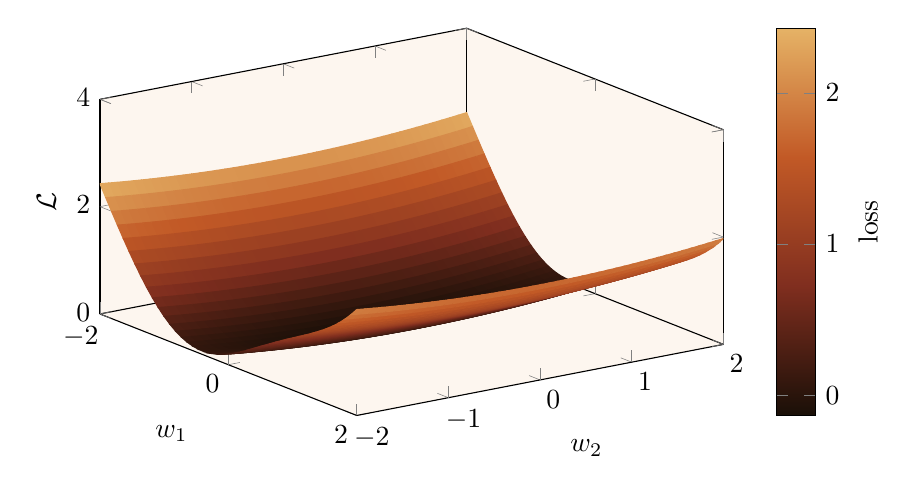
\begin{tikzpicture}
    \begin{axis}[
        width=9.5cm, height=6.5cm,
        xlabel={$w_1$}, ylabel={$w_2$}, zlabel={$\mathcal{L}$},
        view={55}{30},
        domain=-2:2, y domain=-2:2,
        samples=45,
        zmin=0, zmax=4,
        colormap={warm-gradient}{
            rgb(0cm)=(0.1,0.06,0.03)
            rgb(1cm)=(0.5,0.18,0.12)
            rgb(2cm)=(0.76,0.35,0.15)
            rgb(3cm)=(0.9,0.7,0.4)
        },
        axis background/.style={fill=wp-bg},
        colorbar,
        colorbar style={ylabel={loss}}
    ]
        \addplot3[surf, shader=flat] {0.5*x*x + 0.05*y*y + 0.3*sin(2*deg(x))};
    \end{axis}
\end{tikzpicture}
\caption{A slice of a loss landscape. The overall curvature of $w_1$ dominates, but local wrinkles create additional minima, and the shallow $w_2$ direction produces a ravine-like structure.}
\label{fig:loss_landscape}
\end{figure}

The blind hiker metaphor now becomes sharper: the gradient points steepest-uphill \emph{locally}, and the update rule is the hiker's strategy for choosing step sizes in response to the terrain around them.

\subsection{The Training Loop}

The lifecycle of learning is a repetitive cycle:
\begin{enumerate}[leftmargin=*, itemsep=2pt]
    \item \textbf{Forward Pass:} Feed a batch of data through the network to get predictions $\hat{\mathbf{y}}$.
    \item \textbf{Loss Calculation:} Compare $\hat{\mathbf{y}}$ to targets $\mathbf{y}$ using $\mathcal{L}$.
    \item \textbf{Backward Pass:} Run \texttt{backward()} to calculate $\frac{\partial \mathcal{L}}{\partial \theta}$ for all parameters $\theta$.
    \item \textbf{Update:} Adjust the weights using an optimizer.
    \item \textbf{Zero Gradients:} Clear the gradient buffers to prepare for the next batch.
\end{enumerate}

In PyTorch, this translates to the ubiquitous training step:

\begin{lstlisting}[caption={The standard PyTorch training step.}]
optimizer.zero_grad()   # Step 5: Clear old gradients
loss = criterion(y_hat, y) # Steps 1 & 2: Forward and Loss
loss.backward()         # Step 3: Autodiff
optimizer.step()        # Step 4: Update weights
\end{lstlisting}

Why \texttt{zero\_grad()}? In PyTorch, gradients are accumulated by default (due to the sum rule). If we don't clear them, the gradients from step $t$ will be added to the gradients of step $t-1$, causing the network to take artificially large and chaotic steps.

\subsection{Gradient Descent vs. Stochastic Gradient Descent}

\textbf{Batch Gradient Descent} calculates the loss and gradients using the \textit{entire} dataset at once. While mathematically precise (it computes the true gradient of the empirical risk), this is computationally prohibitive for datasets with millions of samples.

\textbf{Stochastic Gradient Descent (SGD)} uses a single random example per update. This is extremely fast but highly noisy. The loss will fluctuate violently, and the path to the minimum will resemble a random walk rather than a straight line.

The industry standard is \textbf{Mini-Batch SGD}. We process a small subset of data (e.g., 32, 64, or 256 samples) per update. This balances the stability of true gradients with the hardware efficiency of parallel matrix multiplications on GPUs.

\begin{table}[htbp]
\centering
\small
\begin{tabularx}{\textwidth}{@{}>{\raggedright\arraybackslash}p{2.6cm}X X X@{}}
\toprule
 & \textbf{Batch GD} & \textbf{Mini-Batch SGD} & \textbf{Stochastic SGD} \\
\midrule
Samples per step & entire dataset & small subset (32--256) & a single sample \\
Gradient quality & exact (true gradient) & low-variance estimate & very noisy estimate \\
Updates per epoch & 1 & $\approx$ samples/batch & samples \\
Speed & slow (one step/epoch) & fast & fastest \\
Stability & very stable, can get stuck & good balance & oscillates a lot \\
GPU efficiency & memory-heavy & excellent (batched matmuls) & poor \\
\bottomrule
\end{tabularx}
\caption{Comparison of gradient descent variants. Mini-batch SGD combines the precision of batch gradients with the throughput of hardware parallelism, making it the default in practice.}
\label{tab:gd_variants}
\end{table}

A useful intuition: the mini-batch gradient is a \emph{noisy estimate} of the true gradient, and the batch size controls the noise level. Smaller batches mean more noise---which can actually help escape shallow local minima and saddle points---but also a more erratic training curve.

\subsection{The Learning Rate}

The learning rate $\eta$ is the single most sensitive hyperparameter in deep learning. It controls the size of each step, and its interaction with the loss landscape determines whether training converges at all.

\begin{figure}[htbp]
\centering
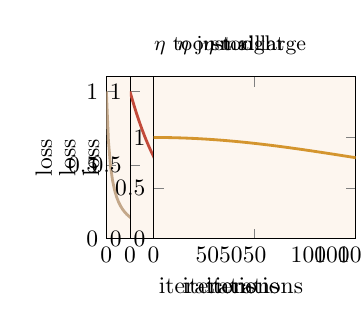
\begin{tikzpicture}[scale=0.85]
    % Panel 1: Too small
    \begin{axis}[
        width=4.6cm, height=4cm,
        xlabel={iterations}, ylabel={loss},
        title={$\eta$ too small},
        ymin=0, ymax=1.1, xmin=0, xmax=100,
        xtick={0,50,100}, ytick={0,0.5,1.0},
        axis background/.style={fill=wp-bg},
        title style={font=\small}
    ]
        \addplot[wp-muted, very thick, domain=0:100, samples=100] {1/(1+0.5*x)};
    \end{axis}
    \hspace{0.3cm}
    % Panel 2: Just right
    \begin{axis}[
        width=4.6cm, height=4cm,
        xlabel={iterations}, ylabel={loss},
        title={$\eta$ just right},
        ymin=0, ymax=1.1, xmin=0, xmax=100,
        xtick={0,50,100}, ytick={0,0.5,1.0},
        axis background/.style={fill=wp-bg},
        title style={font=\small}
    ]
        \addplot[wp-primary, very thick, domain=0:100, samples=100] {exp(-0.05*x)};
    \end{axis}
    \hspace{0.3cm}
    % Panel 3: Too large
    \begin{axis}[
        width=4.6cm, height=4cm,
        xlabel={iterations}, ylabel={loss},
        title={$\eta$ too large},
        ymin=0, ymax=1.6, xmin=0, xmax=100,
        xtick={0,50,100}, ytick={0,0.5,1.0},
        axis background/.style={fill=wp-bg},
        title style={font=\small}
    ]
        \addplot[wp-accent, very thick, domain=0:100, samples=200] {0.8 + 0.2*cos(0.9*x)};
    \end{axis}
\end{tikzpicture}
\caption{Effect of the learning rate on training. Too small $\Rightarrow$ painfully slow convergence; just right $\Rightarrow$ rapid smooth decrease; too large $\Rightarrow$ the loss oscillates or diverges.}
\label{fig:learning_rate}
\end{figure}

A learning rate that is too large can cause divergence: each step overshoots the valley and lands higher up the opposite slope. A rate that is too small wastes compute. This is why modern practice uses \emph{learning rate schedules}---start with a larger $\eta$ and shrink it over time---or adaptive optimizers that effectively tune a per-parameter learning rate (Section~\ref{sec:optimizers}).

\subsection{The Evolution of Optimizers}
\label{sec:optimizers}

Plain SGD updates weights using the rule: $\theta \leftarrow \theta - \eta \nabla_\theta \mathcal{L}$, where $\eta$ is the learning rate. However, the loss landscape of deep neural networks is rarely a perfect bowl; it is full of ravines, saddle points, and flat plateaus. Plain SGD oscillates heavily in ravines (narrow steep valleys) and struggles to escape flat plateaus.

\begin{figure}[htbp]
\centering
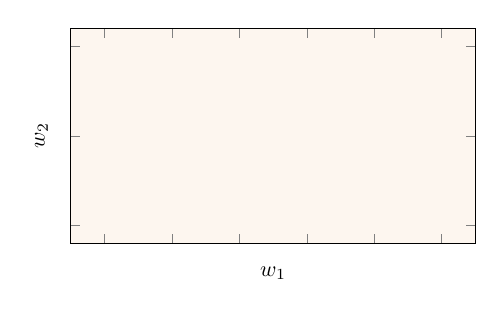
\begin{tikzpicture}[scale=0.8, >=latex]
    \begin{axis}[
        width=8cm, height=5cm,
        xlabel={$w_1$}, ylabel={$w_2$},
        view={0}{90},
        xticklabels={}, yticklabels={},
        colormap={warm-gradient}{
            rgb(0cm)=(0.1,0.06,0.03)
            rgb(1cm)=(0.5,0.18,0.12)
            rgb(2cm)=(0.76,0.35,0.15)
            rgb(3cm)=(0.9,0.7,0.4)
        },
        axis background/.style={fill=wp-bg}
    ]
        % Contour lines simulating a ravine
        \draw[wp-dark!60, line width=0.4pt] (axis cs:0,0) ellipse (2.5 and 0.5);
        \draw[wp-dark!60, line width=0.4pt] (axis cs:0,0) ellipse (2.0 and 0.4);
        \draw[wp-dark!60, line width=0.4pt] (axis cs:0,0) ellipse (1.5 and 0.3);
        \draw[wp-dark!60, line width=0.4pt] (axis cs:0,0) ellipse (1.0 and 0.2);
        \draw[wp-dark!60, line width=0.4pt] (axis cs:0,0) ellipse (0.5 and 0.1);

        % SGD Path (Zig-zag)
        \draw[ultra thick, wp-primary, -latex] 
            (axis cs:1.8, 0.4) -- (axis cs:1.2, -0.3) -- (axis cs:0.8, 0.2) -- (axis cs:0.4, -0.15) -- (axis cs:0.2, 0.08) -- (axis cs:0,0);
        \node[circle, fill=wp-primary, inner sep=1.5pt] at (axis cs:1.8, 0.4) {};
        \node[wp-primary, font=\small\bfseries, above right] at (axis cs:1.8, 0.4) {Start};
        
        % Momentum Path (Smoothed)
        \draw[ultra thick, wp-accent, -latex, dashed] 
            (axis cs:-1.8, 0.4) .. controls (-1.0, 0.1) and (-0.5, 0.0) .. (0,0);
        \node[circle, fill=wp-accent, inner sep=1.5pt] at (axis cs:-1.8, 0.4) {};
        \node[wp-accent, font=\small\bfseries, above left] at (axis cs:-1.8, 0.4) {Start};
    \end{axis}
\end{tikzpicture}
\caption{Optimization in a ravine. Plain SGD (terracotta) oscillates violently across the steep walls. Momentum (gold, dashed) averages out the oscillations, directing the path straight to the minimum.}
\label{fig:sgd_vs_momentum}
\end{figure}

\subsubsection{Momentum}
Momentum addresses the ravine problem by adding physics to the update. Instead of relying solely on the current gradient, it accumulates a velocity vector $v_t$:
\[
v_t = \gamma v_{t-1} + \eta \nabla_\theta \mathcal{L}, \qquad \theta \leftarrow \theta - v_t
\]
Here, $\gamma$ (typically 0.9) acts as friction. If the gradient constantly changes direction (as in the zig-zag in Fig.~\ref{fig:sgd_vs_momentum}), the perpendicular components of $v_t$ cancel out, while the component pointing down the ravine accumulates, accelerating convergence.

Think of a ball rolling down a hill: it does not stop at every bump; it carries \emph{velocity} from previous slopes. The friction coefficient $\gamma$ decides how much past momentum to remember. A small $\gamma$ behaves almost like plain SGD; a $\gamma$ close to 1 (e.g., 0.99) remembers a long history and can overshoot past the minimum, requiring careful tuning. In practice, $\gamma = 0.9$ is a robust default.

\subsubsection{RMSProp (Adaptive Gradients)}
While momentum speeds up the descent, it still uses a global learning rate for all parameters. RMSProp adapts the learning rate for each parameter individually by dividing by the moving average of squared gradients:
\[
v_t = \beta v_{t-1} + (1-\beta)(\nabla_\theta \mathcal{L})^2, \qquad \theta \leftarrow \theta - \frac{\eta}{\sqrt{v_t + \epsilon}} \nabla_\theta \mathcal{L}
\]
If a parameter has consistently large gradients, $v_t$ becomes large, shrinking its effective learning rate. This prevents single parameters from causing destructive updates.

The intuition: some parameters may need large steps while others need tiny ones (e.g., rarely active parameters accumulate small gradients). Dividing each parameter's step by the \emph{root mean square} of its recent gradients normalizes the step sizes across the whole network. The small constant $\epsilon$ (typically $10^{-8}$) prevents division by zero. The decay factor $\beta$ (typically 0.9) controls the window of recent gradients used for normalization.

\subsubsection{Adam (Adaptive Moment Estimation)}
Adam is the default optimizer in modern deep learning. It combines the concepts of Momentum (first moment) and RMSProp (second moment). It maintains an exponential moving average of both the gradients and the squared gradients:
\[
m_t = \beta_1 m_{t-1} + (1-\beta_1)\nabla_\theta \mathcal{L} \quad \text{(First Moment)}
\]
\[
v_t = \beta_2 v_{t-1} + (1-\beta_2)(\nabla_\theta \mathcal{L})^2 \quad \text{(Second Moment)}
\]
Because $m_t$ and $v_t$ are initialized to zero, they are heavily biased toward zero in the early steps. Adam corrects this bias:
\[
\hat{m}_t = \frac{m_t}{1 - \beta_1^t}, \qquad \hat{v}_t = \frac{v_t}{1 - \beta_2^t}
\]
The final update rule is:
\[
\theta \leftarrow \theta - \eta \frac{\hat{m}_t}{\sqrt{\hat{v}_t} + \epsilon}
\]
Adam adapts the learning rate for \textit{each parameter individually}. Parameters that have had large gradients recently will have their learning rate reduced (via division by $\sqrt{\hat{v}_t}$), while parameters with small gradients will take larger steps. This makes Adam incredibly robust across different architectures and hyperparameters.

The bias correction is easy to misunderstand, so it is worth a concrete look. Suppose $\beta_1 = 0.9$ and the very first gradient is $g_1 = 1.0$. Then $m_1 = (1-0.9) \cdot 1.0 = 0.1$---one tenth of the true gradient! The correction divides by $1 - \beta_1^1 = 0.1$, recovering $\hat{m}_1 = 1.0$. Without it, the first few updates would be far too small, artificially slowing the start of training. The default hyperparameters $\beta_1 = 0.9$, $\beta_2 = 0.999$, $\epsilon = 10^{-8}$ work well across almost all problems.

\subsubsection{Choosing an Optimizer}

\begin{table}[htbp]
\centering
\small
\begin{tabularx}{\textwidth}{@{}>{\raggedright\arraybackslash}p{2.2cm}X X X@{}}
\toprule
\textbf{Optimizer} & \textbf{Key Idea} & \textbf{Strength} & \textbf{Weakness} \\
\midrule
\textbf{SGD} & follow $-\nabla \mathcal{L}$ & simple, predictable & slow in ravines; sensitive to $\eta$ \\
\textbf{Momentum} & accumulate velocity & escapes ravines, smooths path & adds $\gamma$; can overshoot \\
\textbf{RMSProp} & per-parameter scaling & handles sparse/skewed grads & relies on good $\beta$ \\
\textbf{Adam} & moments + bias correction & robust default; per-parameter rate & more hyperparameters \\
\bottomrule
\end{tabularx}
\caption{A practical guide to the optimizers covered in this chapter. When in doubt, start with Adam; for fine-tuned convergence or memory constraints, Momentum SGD with a schedule is a strong choice.}
\label{tab:optimizer_guide}
\end{table}

\begin{remark}[The End of the Engine]
We have now completed the core learning mechanism. Our \texttt{mini\_nn} framework can build graphs, compute forward passes, calculate losses, backpropagate gradients, and update weights via Adam. However, we have ignored a critical problem: models with millions of parameters will simply memorize the training data. In Chapter 3, we will address Generalization and Regularization.
\end{remark}

\subsection{Exercises}

\begin{enumerate}[leftmargin=*, itemsep=4pt]
    \item Derive the \texttt{\_backward} function for a new primitive operation, the \emph{sine}: $\frac{d}{dx}\sin(x) = \cos(x)$. Show how you would implement it following the same four-step pattern used in the \texttt{Valor} class.
    \item Trace the backward pass for the expression $L = (x \times y) + x$ with $x = 2$ and $y = 3$ by hand. Note that $x$ appears twice; verify that your result matches the analytic derivative $\frac{\partial L}{\partial x} = y + 1$.
    \item The \texttt{Valor.backward()} method seeds \texttt{self.grad = 1.0} before the loop. Why must the root gradient be seeded, and what would happen if it were initialized to $0$ instead?
    \item Explain, in your own words, why reverse-mode autodiff is used for training while forward-mode would be hopeless. How many forward passes would forward-mode need for a model with $10^6$ parameters and one scalar loss?
    \item Using the sum rule, explain why \texttt{optimizer.zero\_grad()} is necessary in the training loop. What incorrect gradient would a network compute if gradients were never reset?
    \item Compare Batch GD, Mini-Batch SGD, and Stochastic SGD in terms of the noise in their gradient estimates. Which one can help escape a saddle point, and why?
    \item Adam's first moment is initialized to zero and corrected via $1 - \beta_1^t$. Compute $\hat{m}_1$ and $\hat{m}_2$ for $\beta_1 = 0.9$ assuming a constant gradient $g = 1.0$, and confirm that the correction makes the early steps approximately unbiased.
\end{enumerate}

\end{document}